\chapter{Evaluation}
\label{cha:evaluation}

This section demonstrates test evaluations of implemented scenarios to cover the data transmission on the P2P network. The first section introduces the test environment and the evaluation method. The following section describes the results of quantitative and qualitative evaluations by comparing the scenarios. We explain the analysis and discuss about the obtained results.

\section{Test environment}

The test is conducted in a controlled environment. All scenarios used two machines. Table 5.1 describes the machine specification. 

\begin{table}[!ht]
	\small
	\centering
	\begin{tabular}{|l|l|l|l|}
		\hline
		Machine & Soecification & OS & Compiler \\
		\hline
		A01 & Quad core Intel Core i7 2.4Ghz, 8GB RAM & apple-darwin19.6.0 & clang version 12.0.0\\
		\hline
		B01 & AMD FX-8350 8 cores, 4G/Hz, 8GB RAM & Ubuntu 20.04.2 LTS & gcc 10.2.0 \\
		\hline
	\end{tabular}
	\caption{The Machine specification}
\end{table}

All tests are run independently on each machine. The peers are underlying the local network. One of the peers assumes a bootstrap peer. Other peers can establish the connection through the bootstrap peer. A mapping server is deployed for the Staxnet network. The Staxnet network is connected with five peers. There are two buckets because the k-bucket configures up to three peers. The test mainly runs on A01. However, B01 participates in the test under the particular condition.

The test measures following cases

\begin{description}
	\item the uploading and downloading time in the all-peer propagation model. 
	\item the data transmission time using the different protocols in the direct tunnel based P2P model.
	\item QUIC PLMTUD test
\end{description}

In the all-peer propagation model test, a peer conducts to upload and download different sizes of files. The direct tunnel-based P2P model uses different protocols. The test conducts separate measurements for each protocol. The data transmission tests also use different sizes of files. QUIC PLMTUD test is measured comparing different MTU sizes and data transmission time. Using the results of evaluations, we discuss the drawbacks and strong points that were found in the model and we develop methods for improvement.

\section{Measurement methodology}

The model is to be a measured focus on the performance of data transfer in the system. Both models mutually utilize the implementations of the Staxnet daemon. Hence, the transmission time includes the duration of the encryption, decryption, and lookup service. If the traffic congestion occurs in the routing table, the measurement time increases abnormally. In this case, it is classified as an error and needs to be re-measured. Each measurement is performed 50 times, and the result is expressed as the average of these measurements. This measurement takes the data of upload time and download time. The CLI application reads the file in the upload procedure, and then it sends it to the daemon. The given file data are fragmented as a packet; the packet size is fixed with a maximum of 1500 bytes. When the first fragmented packet is sent to the daemon, the time measurement begins. After the routing table update is completed, the daemon sends the state message to the CLI application of the upload procedure. When the CLI application receives this message, the upload time measurement is closed. 

In the download procedure, the CLI application sends the request message to the daemon. The measurement begins. All activities of implementation that are the same as the upload procedure are included in the measurement. However, the direct tunnel-based P2P model executes additional implementation of the retrieval of the address in the mapping server, the tunnel construction, and the handshake between peers. This model includes these procedures. When the CLI application downloads entire packets, the download time measurement is closed.

The data transmission in the test uses four different file sizes: 1 Megabyte, 3 Megabytes, 5 Megabytes, and 10 Megabytes. The direct tunnel-based P2P model measures all protocols, TCP, UDP, and QUIC.

The LSQUIC library supports PLMTUD with IPv6 protocol. The implemented Staxnet network system only supports the IPv4 protocol. For this experimental test, we use the single file transmission application. This implementation is developed using the given sample application, and it is the base model of the QUIC transmission part in the direct tunnel-based P2P model. Because of this reason, this is - in the implementation section. Moreover, Mac OS does not support the ‘Don’t Fragment’ flag. This test is conducted in the B01 machine. We have designed it separately using set MTU size as 1500 bytes and 5000 bytes, and three different sizes of the file are transmitted as 5, 10, and 20 Megabytes.

\section{Measurement results}

First, we evaluate the results of all peer propagation model. Figure 5.1 shows the file transmission times. In this graph, the upload and download time are expressed. As the file First, we evaluate the results of all peer propagation model. Figure 5.1 shows the file transmission times. In this graph, the upload and download time are written. As the file size increased, the transmission time taken also has increased accordingly. These times include the transmission between the CLI application and the daemon, memorial DB storage, crypto service, and routed list of the bucket. The point to note in this graph is that the upload time took twice as long as the download time. In the Staxnet DHT network, the key-value pair is propagated to the peers in the bucket, and the value is the set of entire packets. Therefore, the system reads the whole file when the key-value pair is stored. The overload occurs when the file is uploading rather than downloading.

\begin{figure}[!ht]
	\centering
	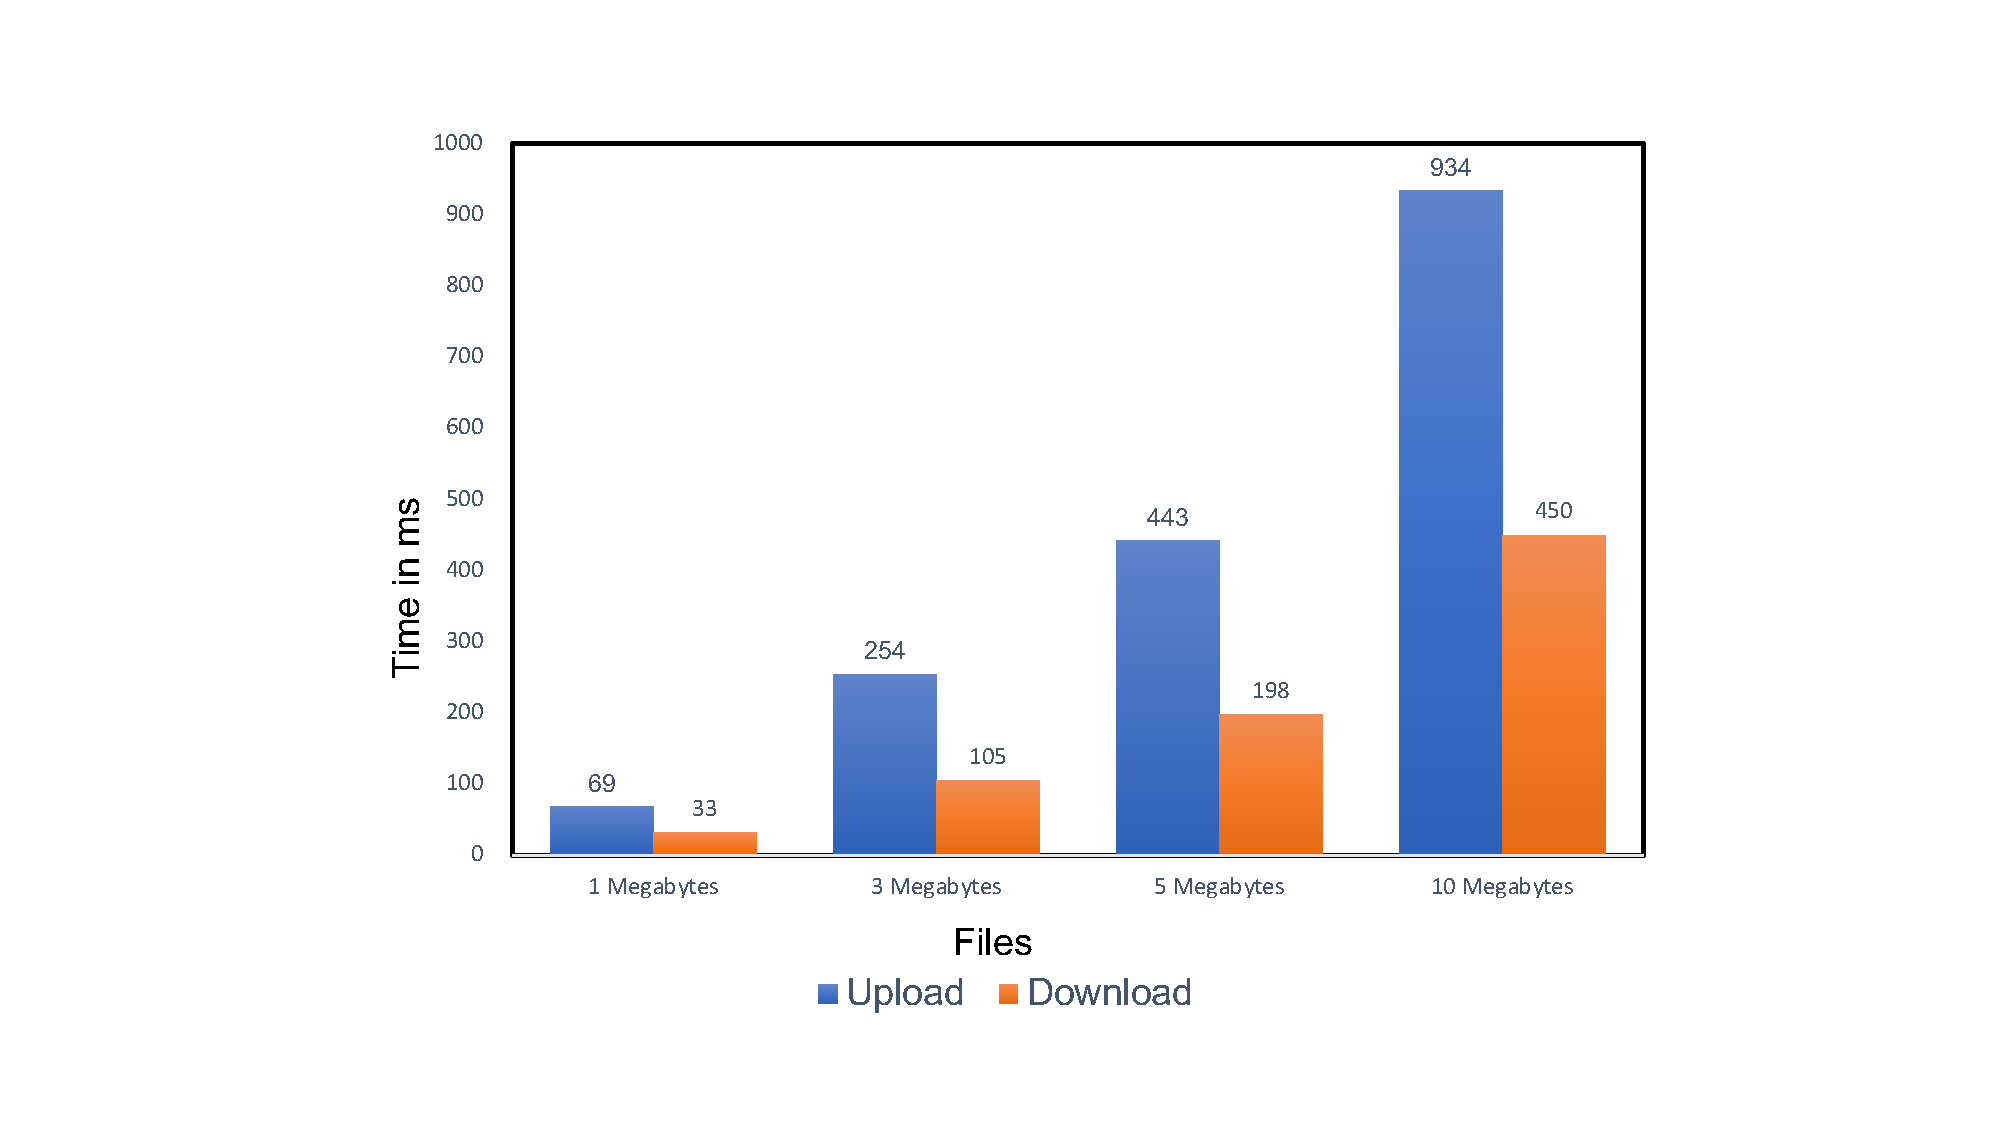
\includegraphics[width=0.5\textwidth]{images/fig_5_1.pdf}\\
	\caption{The file transmission time of the all peers propagation model}
	\label{fig:allpeers}
\end{figure}

Figure 5.2 displays the file download time of the direct tunnel-based P2P model. It appears that the transmission times using TCP, UDP, and QUIC are different for each file sizes. It shows dramatic results compared to the other model. Both models have no difference when they transmit a file smaller than 1 Megabyte. However, in the large file transmission, this model shows fast performances in all protocols. Before proceeding with this test, we predict that the transmission using the UDP protocol is faster than the TCP protocol because the feature of TCP is the 3+1-RTT handshake, including crypto handshake. As a result, the UDP protocol shows faster performance, but it is not significant. The most striking result of this test is QUIC. The results  overwhelmingly shows that large file transfers are about three times faster than other protocols. The QUIC protocol can be a good alternative for large file transfers.

\begin{figure}[!ht]
	\centering
	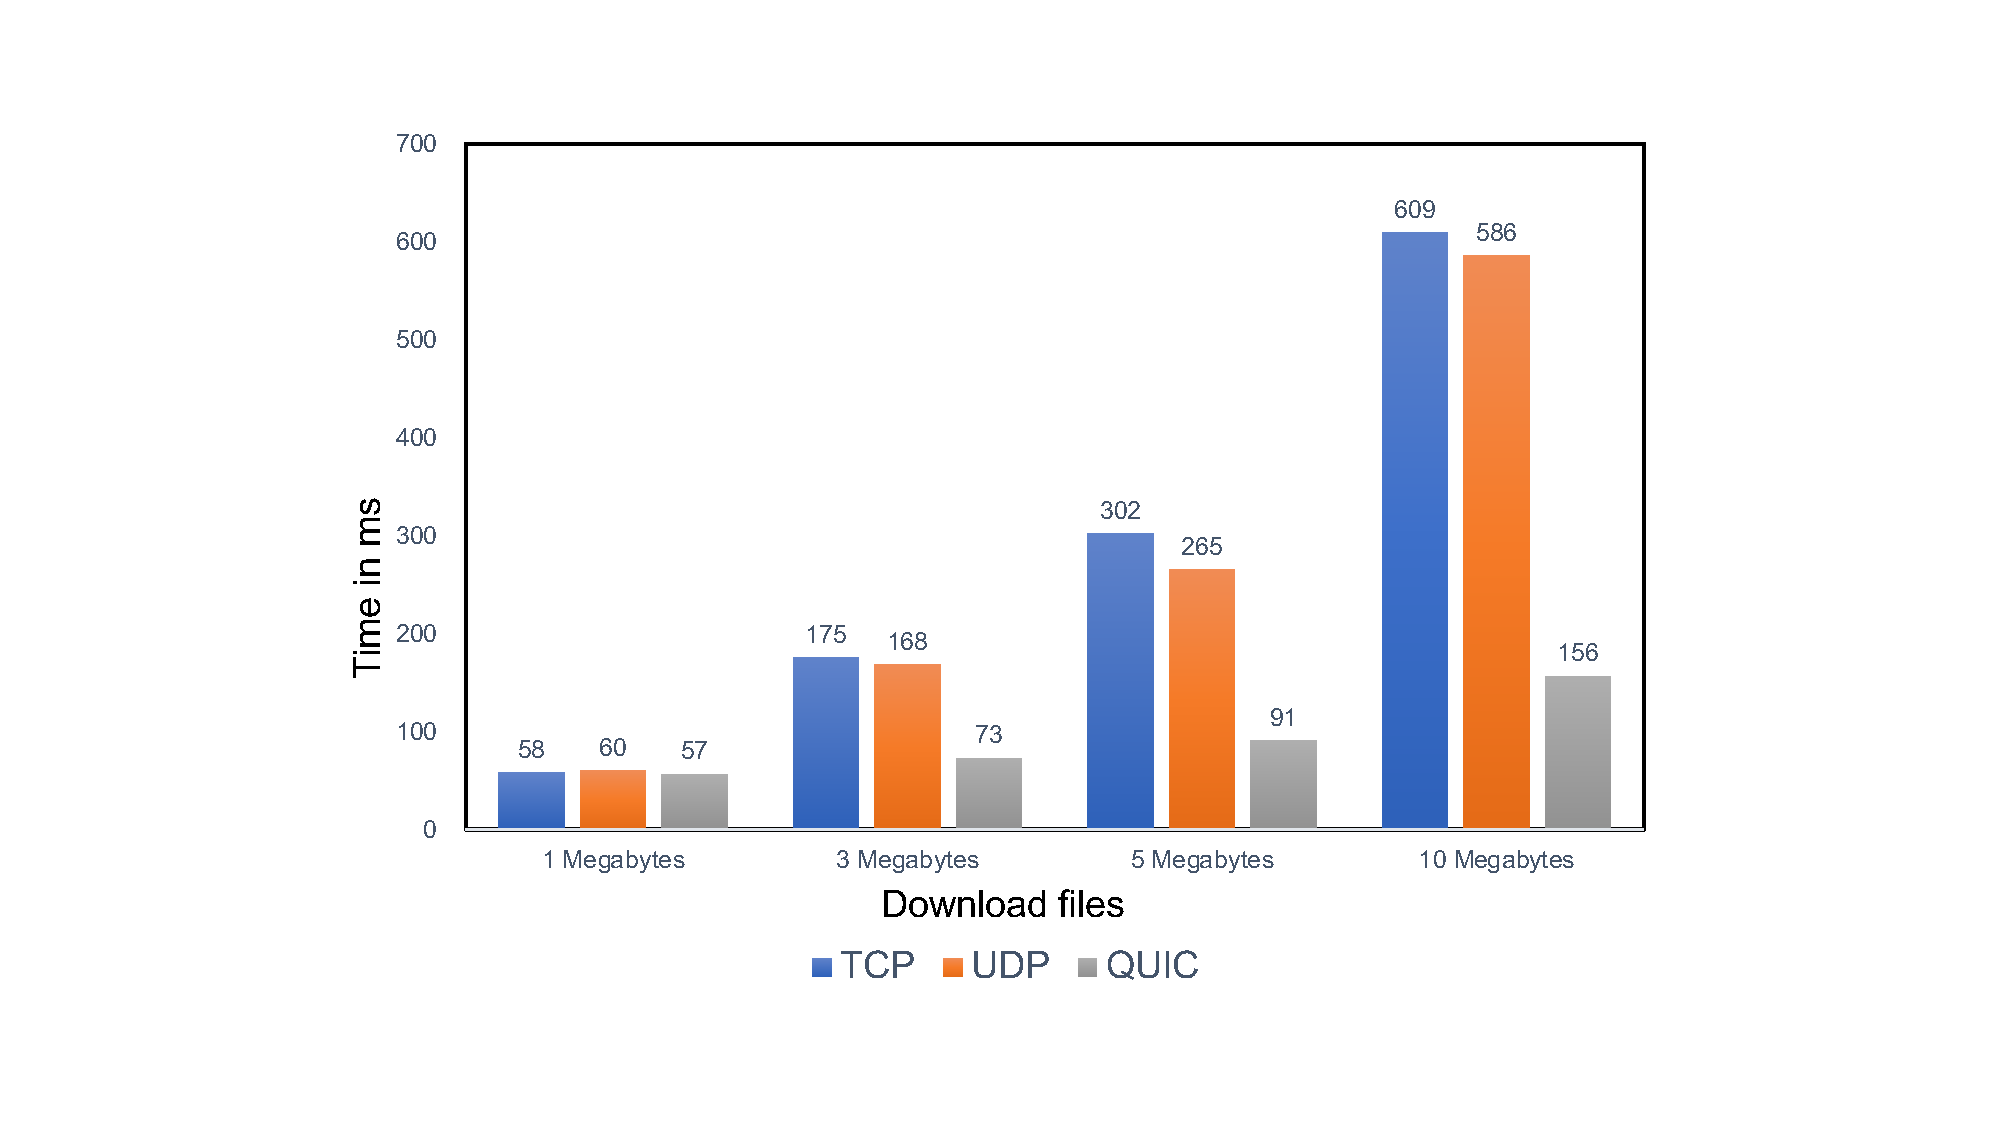
\includegraphics[width=0.5\textwidth]{images/fig_5_2.pdf}\\
	\caption{The file download time of the direct tunnel-based P2P model}
	\label{fig:t_download}
\end{figure}

Figure 5.2 displays the file download time of the direct tunnel-based P2P model. It appears that the transmission times using TCP, UDP, and QUIC are different for each file sizes. It shows dramatic results compared to the other model. Both models have no difference when they transmit a file smaller than 1 Megabyte. However, in the large file transmission, this model shows fast performances in all protocols. Before proceeding with this test, we predict that the transmission using the UDP protocol is faster than the TCP protocol because the feature of TCP is the 3+1-RTT handshake, including crypto handshake. As a result, the UDP protocol shows faster performance, but it is not significant. The most striking result of this test is QUIC. The results  overwhelmingly shows that large file transfers are about three times faster than other protocols. The QUIC protocol can be a good alternative for large file transfers.

Figure 5.3 illustrates the upload time of this model. In this result, there are two noticeable characteristics. First, there is no apparent distinction between the protocols. Second, this model is quite fast, making it hard to compare with the all-peers propagation model. The reason lies in the size of the value. This model uses the value as the peer's identifier. The \textit{node\_id} is only 32 bytes. This model’s payload, including the key-value pair, is comprised of the header with a maximum of 184 bytes and a payload with a minimum of 33 bytes; the key is a file name. Because of this reason, it can be uploaded to the network.

\begin{figure}[!ht]
	\centering
	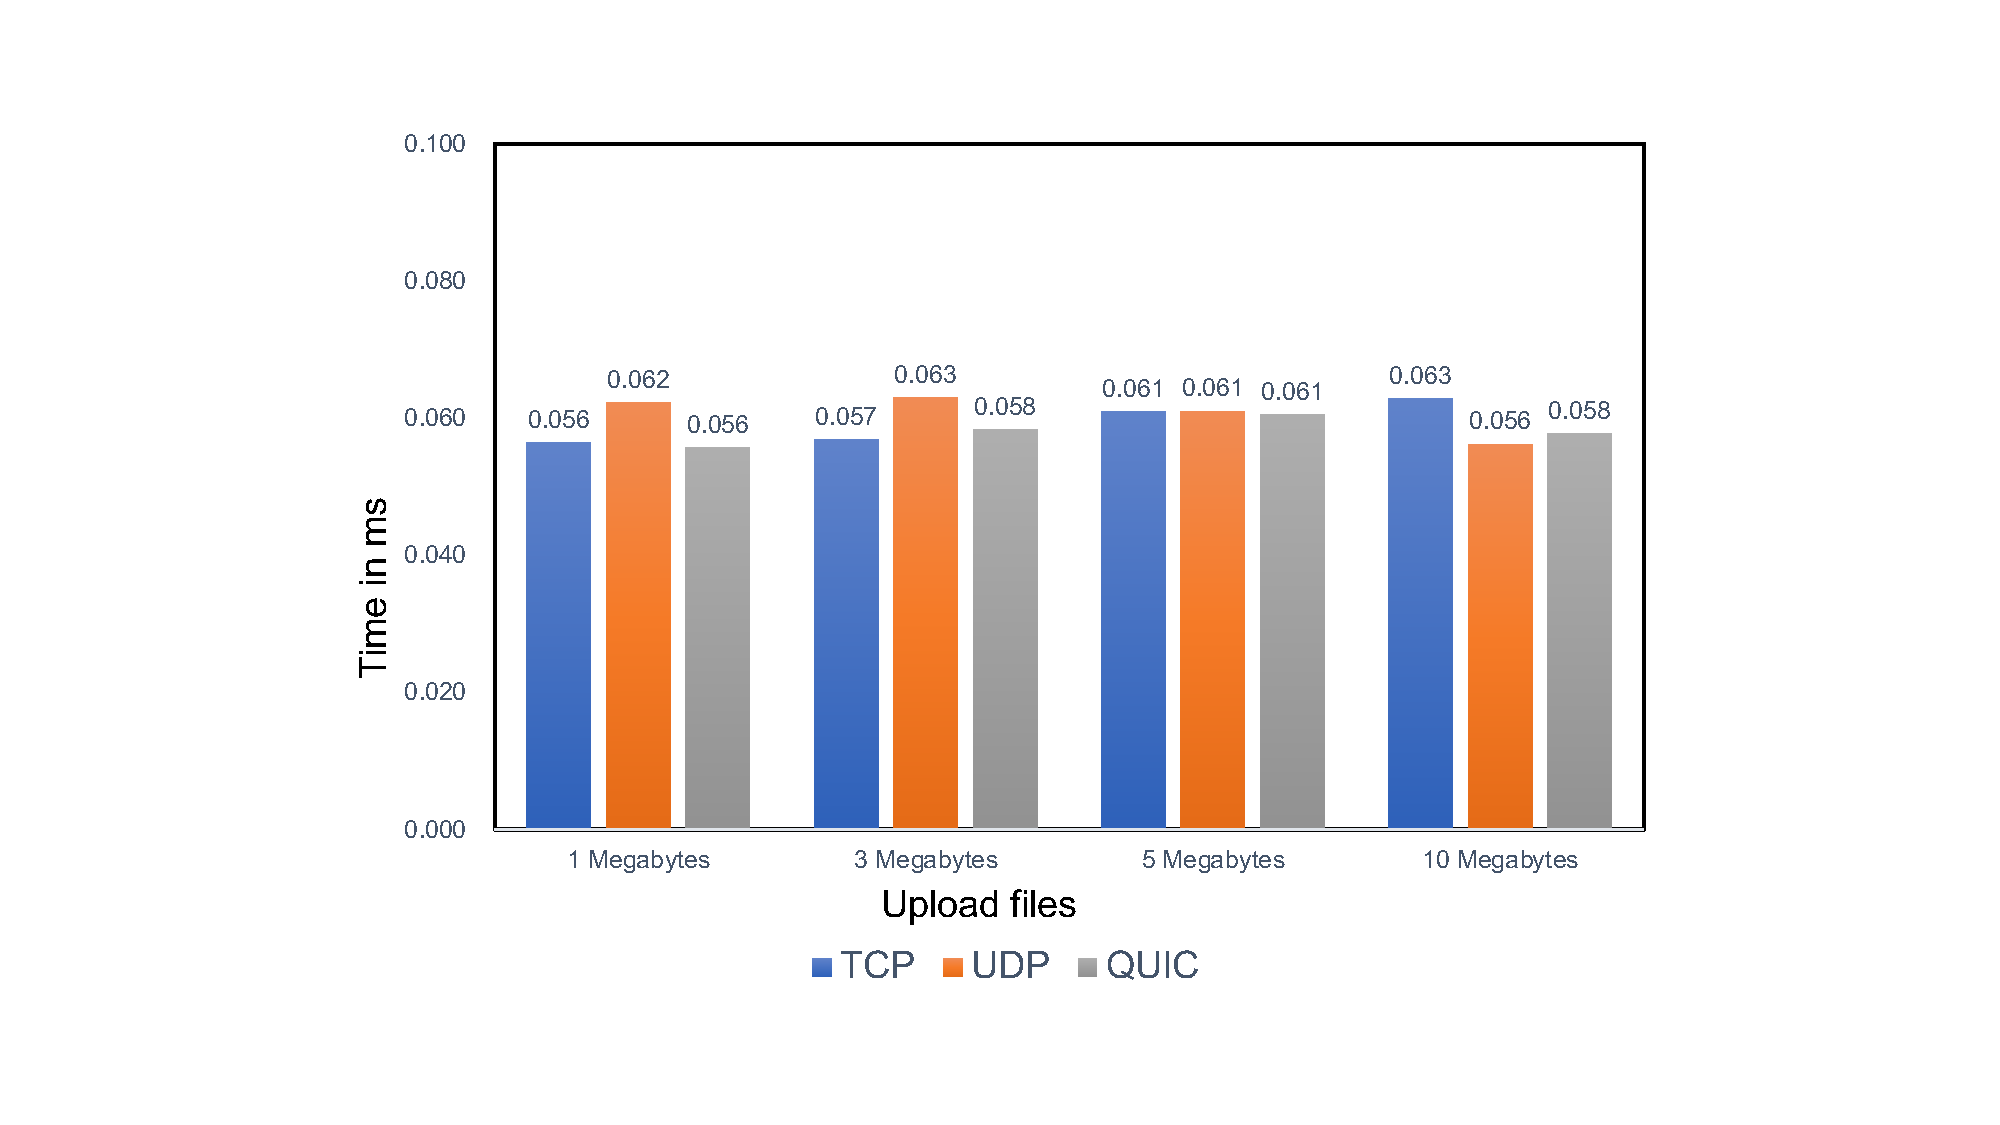
\includegraphics[width=0.5\textwidth]{images/fig_5_3.pdf}\\
	\caption{The file upload time of the direct tunnel-based P2P model}
	\label{fig:t_upload}
\end{figure}

The last result of the evaluation is the experimental data transmission case. Figure 5.4 shows the change of transmission speed according to MTU size. We want to know the effect of a larger MTU size on the data transmission. It was tested by increasing the MTU size by about 2.3 times. It can be seen that the data transfer rate is about 30\% faster. However, this performance cannot be expected to occur in the real world because the large packet over the MTU size is not possible for transmission

\begin{figure}[!ht]
	\centering
	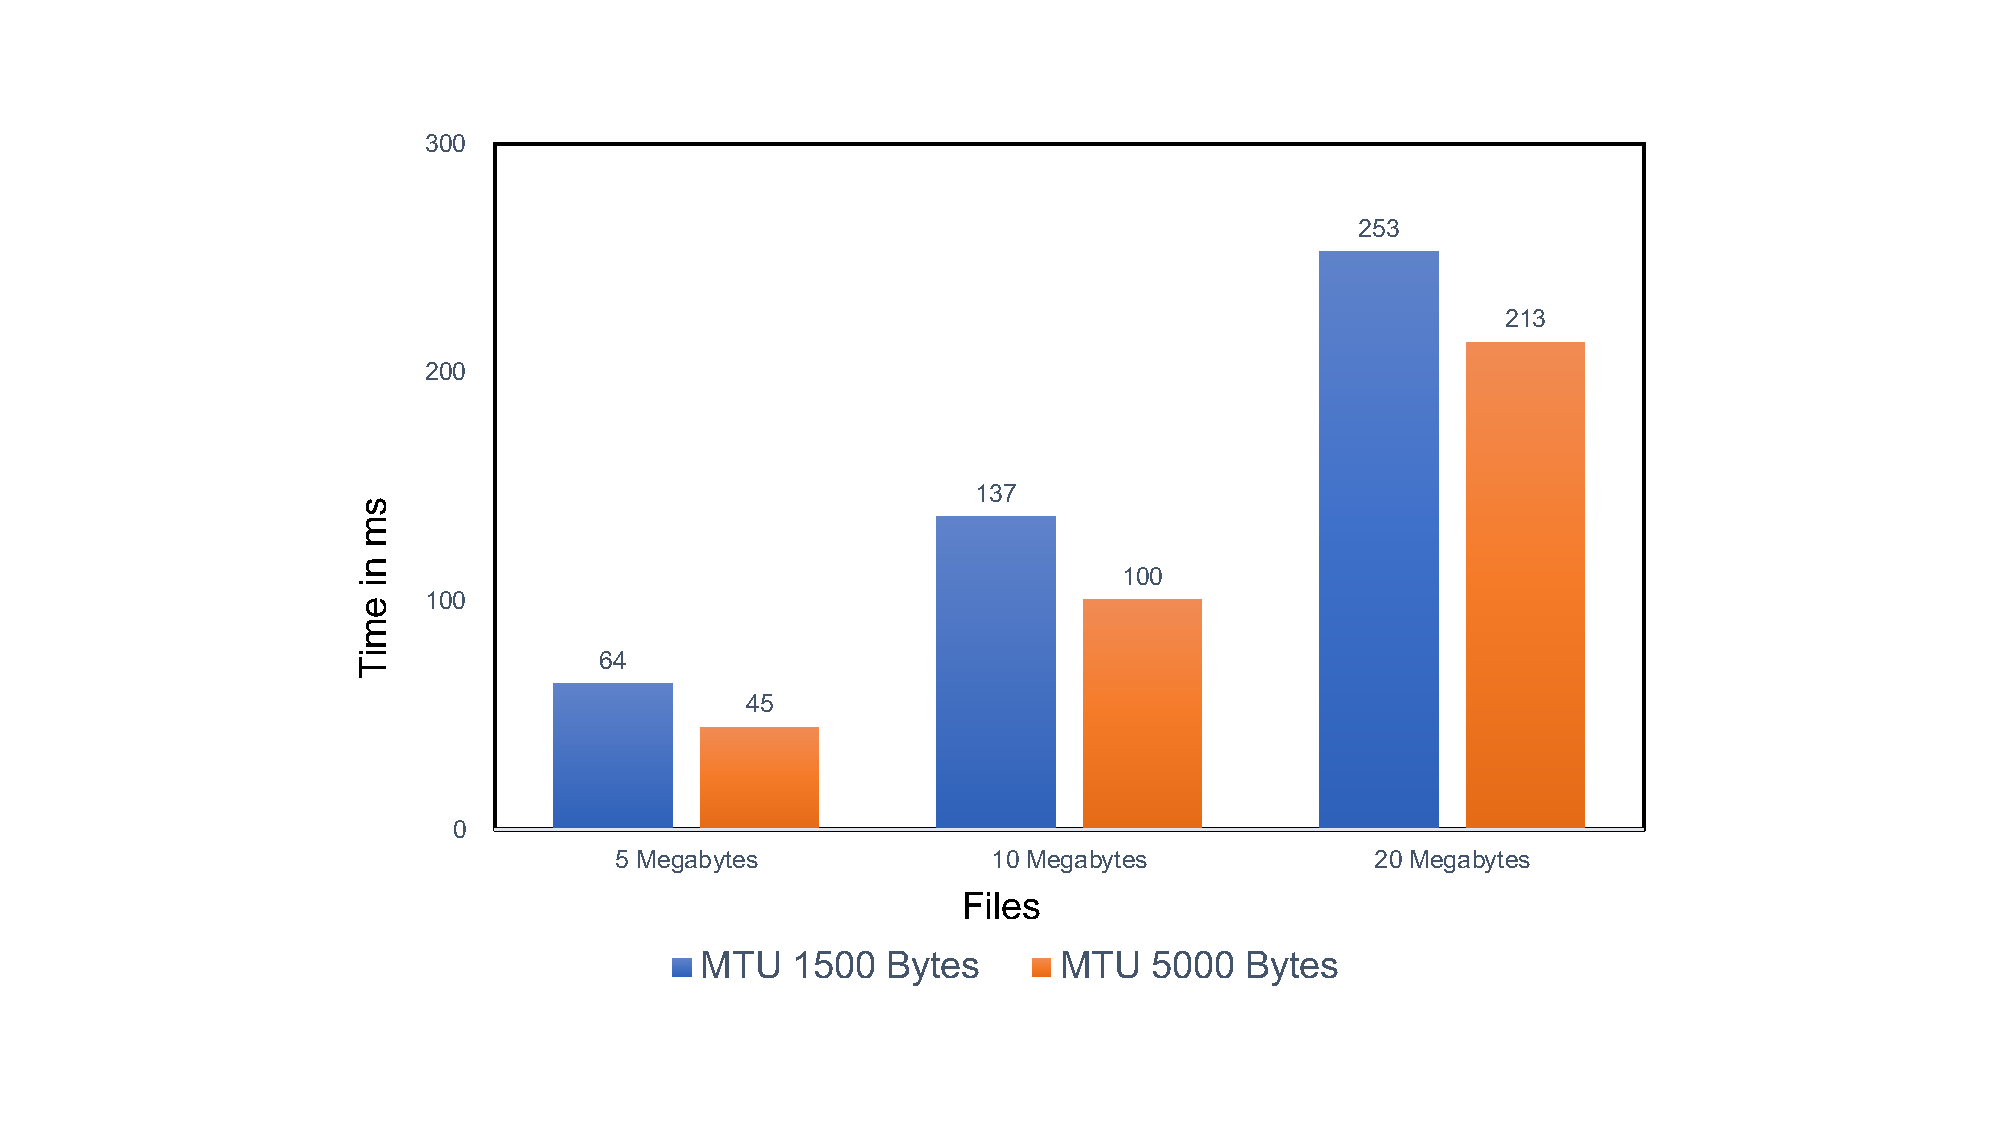
\includegraphics[width=0.5\textwidth]{images/fig_5_4.pdf}\\
	\caption{The change of transmission speed according to MTU size}
	\label{fig:MTU size}
\end{figure}

\section{Analysis and discussion}

With the results obtained from the measurements, we analyze the system comparing both models. The Kademlia DHT P2P network system shows good performance in file sharing. Because the two models processing small data have no remarkable differences in performance, the Kademlia DHT is reliably processed in the system. However, the existing model has the disadvantage of large data sharing. When a key-value pair is routing the peers in the bucket, the network traffic increases with the value amount. Thus, the direct tunnel-based P2P model is stable in large data sharing.

The investigation of the data transmission using the QUIC protocol shows the potential for advancing network performance. The transmission speed certainly distinguishes it from other protocols. However, it is not standardized yet and requires the adoption of external libraries. In the secure aspect, when the critical secure problem occurs from the external library, the system is technically an incompetent state. It is challenging to deploy the new protocol to the overall existing system.

In conclusion, with the results, we can gain the best method in the large data transmission. When the DHT P2P network uses the small size of the propagated key-value pair in the direct tunnel-based P2P model, the upload time takes on average 0.05 milliseconds. In the file with the share of 10 Megabytes, the QUIC protocol is faster than other protocols (being about 70\%). Therefore, this model gives great benefits for large data transmission.
